\chapter{Why Many-core? CPUs versus GPUs}
\label{ch:manycore}

\slides{2--3}

Part~I of these notes was about machines with a handful to a few hundred big, independent
processors. This second part is about a very different design: a chip with \emph{thousands} of
small, simple arithmetic units, the \term{many-core} processor. The most important example is the
\term{GPU} (Graphics Processing Unit). Almost every large machine-learning model and a large share of
the world's fastest supercomputers run on GPUs, so the architecture is worth understanding properly.

\section{From drawing pictures to general computing}

The slide says that GPUs were \emph{``primarily proposed for graphics applications''} and that
graphics \emph{``consists of stages with each stage consisting of independent computations''}.
Let us unpack this, because it explains the whole design.

To show a frame of a game, the computer must decide the colour of every pixel of the screen. A
$1920\times1080$ screen has about $2$ million pixels, and a new frame is needed $60$ times per second. The work per pixel is
a small program (find the surface visible at that pixel, work out the lighting, look up a texture,
blend colours). The key observation is:
\begin{keyidea}
The colour of one pixel does not depend on the colour of any other pixel in the same frame. Millions of
tiny, \emph{independent} jobs can therefore run at the same time, with no communication between them.
\end{keyidea}

The graphics work is organised as a \emph{pipeline} of stages: first the geometry of the scene
(triangles) is transformed into screen coordinates (one independent job per vertex), then triangles
are turned into pixels (one job per triangle), then each pixel is shaded (one job per pixel), and
finally the pixels are written into the frame buffer. Within every stage the jobs are independent;
only between stages is there an order. This is exactly the kind of workload for which you
want as many arithmetic units as possible, each doing the same small program on different data.

Engineers noticed that the same hardware could do other independent computations: multiplying
matrices, simulating physics on a grid, training neural networks. Using a graphics chip for
non-graphics work is called \term{GPGPU} (general-purpose computing on GPUs), and it is what we
study here.

\section{Two design philosophies}

\subsection{What a CPU core is built for}

The slide gives a number: a single CPU chip can have \emph{up to} about $128$ cores (this
figure grows from year to year; the point is the order of magnitude, tens to a couple of hundred). Each CPU core is a
large and sophisticated machine. In Part~I we met several of its tricks: deep pipelines,
out-of-order execution and speculation for instruction-level parallelism, and large multi-level caches
(Chapter~\ref{ch:coherence}). All of these exist for one purpose: to make \emph{one thread of instructions} finish
as quickly as possible, i.e.\ to minimise \term{latency}. The price is that most of the transistors
on a CPU core are spent on control logic and cache, not on arithmetic.

\subsection{What a GPU core is built for}

A GPU does the opposite. Its cores are \term{light-weight}: no speculation, no out-of-order machinery,
and tiny caches per core. In the space of one big CPU core one can place many simple arithmetic units.
The GPU does not try to make any \emph{one} thread fast. It tries to finish the \emph{total} work
quickly by running a huge number of threads at once, i.e.\ to maximise \term{throughput}.

\begin{definition}{latency and throughput}
\term{Latency} is the time one task takes from start to finish (seconds per task).
\term{Throughput} is the number of tasks, or the amount of work, finished per unit time (tasks per second).
They are not opposites, but a design optimised for one is usually not optimal for the other.
\end{definition}

\begin{intuition}
A sports car and a bus. The car has low latency for one passenger (it gets that person there
quickest). The bus is slow, but it moves $50$ people at once, so it has higher throughput. If you
must move $10\,000$ people from one stadium to another, you want buses. A CPU is the sports
car. A GPU is a fleet of buses.
\end{intuition}

\begin{figure}[ht]
\centering
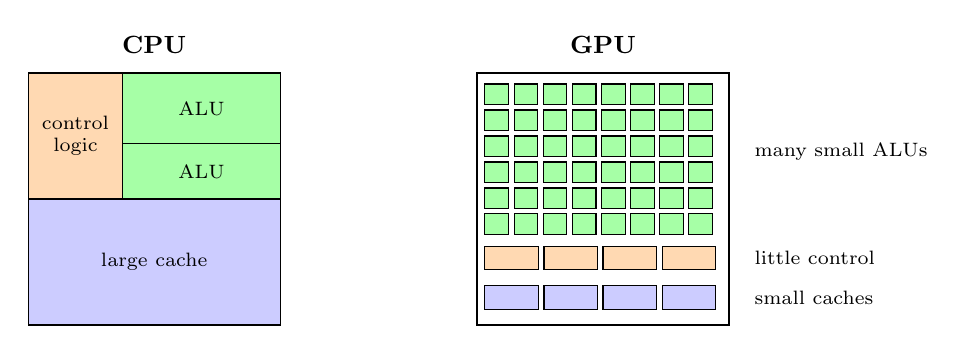
\begin{tikzpicture}[font=\scriptsize]
  % CPU
  \node at (1.6,3.55) {\small\textbf{CPU}};
  \draw (0,0) rectangle (3.2,3.2);
  \draw[fill=orange!30] (0,1.6) rectangle (1.2,3.2) node[midway,align=center] {control\\logic};
  \draw[fill=green!35] (1.2,2.3) rectangle (3.2,3.2);
  \draw[fill=green!35] (1.2,1.6) rectangle (3.2,2.3);
  \node at (2.2,2.75) {ALU};  \node at (2.2,1.95) {ALU};
  \draw[fill=blue!20] (0,0) rectangle (3.2,1.6) node[midway] {large cache};
  % GPU
  \node at (7.3,3.55) {\small\textbf{GPU}};
  \draw (5.7,0) rectangle (8.9,3.2);
  \foreach \i in {0,...,7}{\foreach \j in {0,...,5}{\draw[fill=green!35] (5.8+0.37*\i,1.15+0.33*\j) rectangle +(0.3,0.26);}}
  \foreach \i in {0,1,2,3}{\draw[fill=orange!30] (5.8+0.75*\i,0.7) rectangle +(0.68,0.3);}
  \foreach \i in {0,1,2,3}{\draw[fill=blue!20] (5.8+0.75*\i,0.2) rectangle +(0.68,0.3);}
  \node[anchor=west] at (9.1,2.2) {many small ALUs};
  \node[anchor=west] at (9.1,0.85) {little control};
  \node[anchor=west] at (9.1,0.35) {small caches};
\end{tikzpicture}
\caption{Schematic split of chip area (not to scale; an original illustration of the general idea).
A CPU spends most of its area on control logic and cache to speed up a few threads;
a GPU spends most of its area on arithmetic units.}
\label{fig:cpugpu}
\end{figure}

\begin{pitfall}
``Core'' does not mean the same thing on a CPU and a GPU. A CPU core can fetch, decode and run its own instruction stream. A
GPU ``CUDA core'' (see Chapter~\ref{ch:a100}) is just an arithmetic unit; it cannot decide
what to execute by itself. When comparing ``$128$ cores'' with ``$6912$ cores'', you are comparing
a complete processor with a single floating-point unit. Never compare these numbers directly.
\end{pitfall}

\subsection{What kind of programs suit a GPU?}

Because of its design, a GPU shines when the program has:
\begin{enumerate}
  \item \textbf{lots of data parallelism}: the same operation applied independently to many data elements
        (vector addition, matrix multiplication, image filters, neural-network layers);
  \item \textbf{high arithmetic intensity}: many arithmetic operations for every byte fetched from memory (Chapter~\ref{ch:gpumem});
  \item \textbf{regular control flow}: threads that run next to each other take the same branches (Chapter~\ref{ch:a100}).
\end{enumerate}
It performs poorly on a program that is mostly a single long chain of dependent steps (a
parser, a recursive search), because there is nothing to spread over thousands of units and the
individual GPU threads are slow.

\section{Heterogeneous computing: CPU and GPU together}

\slides{3}

The slide says that \emph{``typically GPU and CPU coexist in a heterogeneous setting''}.
\begin{definition}{heterogeneous system}
A computer that contains processors of \emph{different kinds}, here a CPU (the \term{host}) and
one or more GPUs (the \term{devices}), each used for the work it is best at.
\end{definition}

The slide's division of labour is: the ``less'' computationally intensive part runs on the CPU, and the more intensive parts run on the GPU.
It also labels these two kinds of parallelism:
\begin{itemize}
  \item \term{Coarse-grained} parallelism: a few big, long-running tasks, each doing a lot of work between synchronisations. This matches the CPU's few strong cores.
  \item \term{Fine-grained} parallelism: a very large number of tiny tasks (even one array element each). This matches the GPU's thousands of weak units.
\end{itemize}

A typical program therefore looks like this:
\begin{enumerate}
  \item The CPU runs the main program: reads input, sets things up, and does the serial parts.
  \item The CPU copies the data that the GPU needs from its own memory to the GPU's memory
        (over the PCIe bus, or NVLink).
  \item The CPU \emph{launches a kernel}, a function that runs on the GPU in many threads at once.
  \item The GPU works. Meanwhile the CPU may do other things.
  \item The CPU copies the results back and carries on.
\end{enumerate}

\begin{pitfall}
Step~2 and step~5 are not free. The GPU has its own separate memory; the CPU and GPU do not
share an address space by default (compare the distributed-memory machines of Chapter~\ref{ch:classify}!).
Moving data over the host--device link is much slower than the GPU's own memory. So a computation is only worth sending to the GPU if the speed-up it gets from the many cores is larger than the cost of the transfer.
\end{pitfall}

\begin{workedex}{is offloading worth it?}
Suppose a task needs $2$~GB of input, and the host--device link moves about $25$~GB/s (a typical PCIe~4.0 $\times16$ link: assumed numbers for illustration).
The copy takes $2/25=0.08$~s. If the CPU alone needs $0.3$~s and the GPU needs only $0.02$~s for the computation,
then the GPU path costs $0.08+0.02=0.10$~s (and the results must also be copied back), against $0.3$~s on the CPU:
still worth it. But if the CPU needed only $0.09$~s, offloading would lose, even though the
GPU kernel itself is $4.5\times$ faster than the CPU.
\end{workedex}

\section{NVIDIA and CUDA}

The slide continues: \emph{``NVIDIA's GPU architecture is called CUDA (Compute Unified Device Architecture)
architecture, accompanied by CUDA programming model, and CUDA C language''}. CUDA is therefore three things at once,
and it helps to keep them apart:
\begin{enumerate}
  \item the \textbf{hardware architecture}: how the chip is organised (Chapters~\ref{ch:a100}--\ref{ch:gpumem});
  \item the \textbf{programming model}: the way a programmer describes parallel work (grids, blocks, threads, memory spaces); this is the topic of the later CUDA lectures;
  \item the \textbf{language and tools}: CUDA~C/C++ extends C with a few keywords, and a compiler (\cl{nvcc}) builds both CPU and GPU code from one source file.
\end{enumerate}
The picture on the slide contrasts a $4$-core CPU with a $240$-core GPU of an older generation. Today's numbers are much larger
(Chapter~\ref{ch:a100}), but the ratio of ``a few strong cores'' to ``hundreds or thousands of weak ones'' is the point.

\section*{Exercises}
\begin{enumerate}[label=\textbf{\thechapter.\arabic*},leftmargin=*]
  \item In your own words, why can a graphics workload keep thousands of arithmetic units busy? Give one non-graphics example with the same property.
  \item Explain the difference between latency and throughput using a CPU thread and a GPU thread as the two examples.
  \item A colleague says ``a GPU with $6912$ cores is $54$ times better than a CPU with $128$ cores.'' Give two reasons why this comparison is not meaningful.
  \item For which of these would you expect a GPU to help a lot, and for which not? Explain briefly. (a) Adding two arrays of $10^{8}$ numbers. (b) Walking a linked list of $10^{6}$ nodes. (c) Applying a blur filter to a $4000\times3000$ image. (d) Computing the $n$-th Fibonacci number by the plain loop.
  \item The input is $4$~GB and the link bandwidth is $16$~GB/s. The results are $1$~GB. A CPU does the whole job in $1.0$~s; the GPU kernel takes $0.2$~s. Is offloading worthwhile (ignore overlap of copy and compute)? What is the speed-up?
  \item Distinguish coarse-grained from fine-grained parallelism. Which one does the GPU promote, and which one does the host CPU?
\end{enumerate}
